\documentclass[12pt]{../notes}

% Command for Questions
%\question{}

% Command for Notes
% \note{}

% Code to create a minipage where you can type in class notes. 
%%\begin{minipage}[l][2cm][c]{\textwidth}
%\begin{comment}

%\end{comment}
%%\end{minipage}


% Begin Document
%==============================================================================
\begin{document}
% Include the Title of the Handout
\ntitle{5.2. Nominal/Ordinal Logistic Regression}

\question{Name one potential advantage and one potential disadvantage for using a nominal logistic regression model to describe an ordinal categorical variable?}

\begin{minipage}[l][4cm][c]{\textwidth}
%\begin{comment}
\note{\begin{itemize}
\item \textbf{Advantage:} No longer have to worry about assumption of proportional odds (i.e. the increase in odds for a change in X is constant regardless of the desired category level).
\item \textbf{Disadvantage:} You compute more coefficients than you need to (as no parameter estimates are shared between models). 
\end{itemize}}
%\end{comment}
\end{minipage}

\nspace 
\question{Given the nominal logistic regression output in Figure \ref{fig:logit_output} and obtained from 5.2.1, please write out the two polytomous logistic regression equations.}

\begin{minipage}[l][3cm][c]{\textwidth}
%\begin{comment}
\note{
\begin{align*}
L_{2|1} &=  -0.591 - 0.388*\text{sex} + 1.128*\text{age}_2 + 1.588*\text{age}_3 \\
L_{3|1} &=  -1.039 - 0.813*\text{sex} + 1.478*\text{age}_2 + 2.917*\text{age}_3 \\
\end{align*}
}
%\end{comment}
\end{minipage}

\nspace 
\question{What is the estimated probability that a 30 year old woman will rate AC and Power Steering as a ``very important'' feature?}

\begin{minipage}[l][4cm][c]{\textwidth}
%\begin{comment}
\note{
\begin{align*}
L_{2|1} &=  -0.591 + 1.128 = 0.537 \\
L_{3|1} &=  -1.039 + 1.478 = 0.439 \\
\hat{\pi} &= \frac{e^{0.439}}{1+e^{0.537} + e^{0.439}} = 0.364 
\end{align*}
36.4\%}
%\end{comment}
\end{minipage}


\begin{figure}[H]
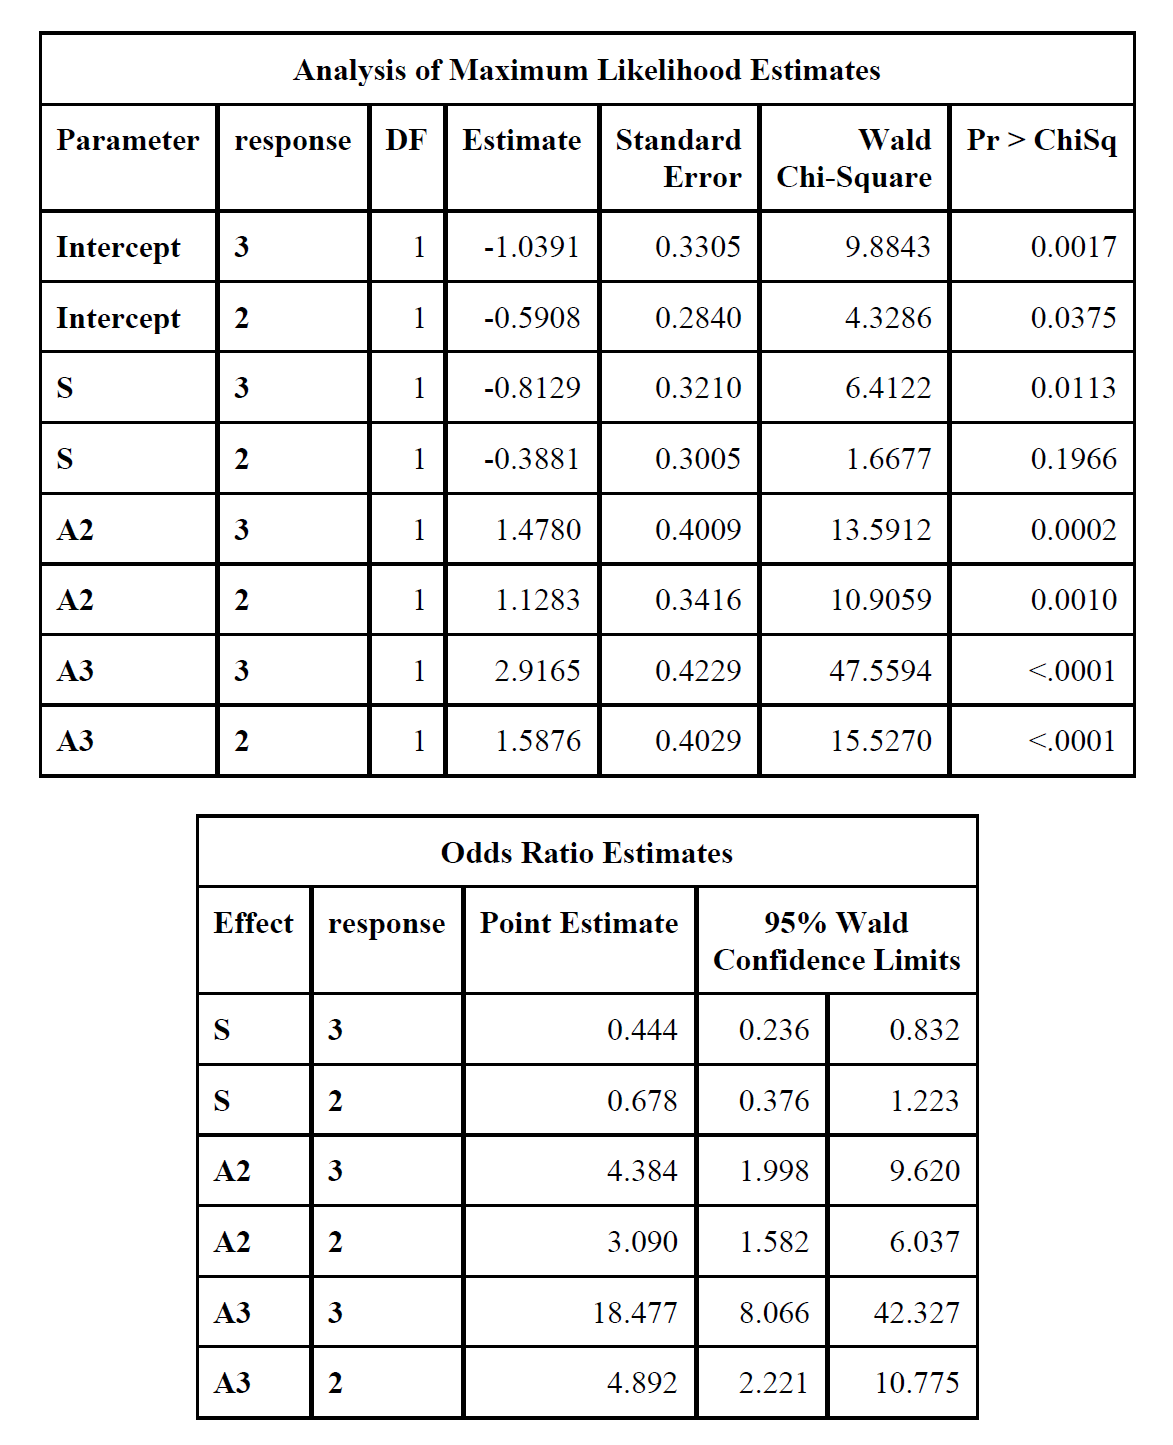
\includegraphics[width=\textwidth]{../figures/module5/multi_logistic_regression.png}
\caption{Nominal logistic regression models using age and sex to predict odds of rating AC and power steering in cars as not important/important/very important.}
\label{fig:logit_output}
\end{figure}





% End the Document
%==============================================================================
\end{document}